\documentclass{article}
\usepackage{url}
\usepackage{graphicx} % To include figures
\usepackage{caption}
\usepackage{fullpage}
\usepackage{subcaption}
\usepackage{fancyvrb} % Includes the \VerbatimInput command to read in code files
\usepackage{float}        % So we can put a figure RIGHT FUCKING HERE

\graphicspath{ {images/} }

% A very simple environment for writing pseudo-code
\newenvironment{pgm}{
  \begin{center}\begin{tabbing}
  xx \= xx \= xx \= xx \= xx \= xx \= xx \= xx \= xx \= xx \= xx \= \kill\>\+}{
  \end{tabbing}\end{center}}

\begin{document}
\begin{center}
	{\scshape \LARGE Examining New York City's Yellow Taxi Data Set \par}
	\vspace{0.3cm}
	{\scshape \large CS 516 Final Project - Midterm Report\par}
	\vspace{0.3cm}
	{ Ziyi \textsc{Wang}, Timothy \textsc{Blumberg}\par}
	\vspace{0.3cm}
	{ October 28, 2016\par}
	\vspace{1.5cm}
\end{center}

\section*{Abstract}

In our final project, we analyze NYC's {\textit very} public taxi dataset \cite{dataset} for interesting and surprising results. Our analysis has been principally done through queries on a SQL database, but because of the geographic nature of the data, we were forced to visualize from a very early stage in our project's formation. During this preliminary stage of developing our project, we have established an efficient workflow and found areas to engage in a more prolonged analysis during the remainder of the semester.

\section{The Data}
The dataset is extremely large (there is about $1.6$Gb of data produced every month at present date), so this creates many challenges as we attempt to gain insights from it. A powerful DBMS helps to cut down our query runtime considerably. The data is relatively clean given its size and complexity, and definitions for the coded portions of the data (such as the {\tt payment\_type} field) is given in the data dictionary \cite{dictionary}. The NYC Taxi \& Limousine Commission (TLC) collects and reports data for three different kinds of vehicles in NYC: yellow taxis, green taxis, and for-hire vehicles (FHV). Yellow taxis provide street-hailing service in Manhattan, Green taxis are designed to be useful when getting around in the boroughs of NYC, and the FHVs are available only through pre-arranging the pickup (i.e. cannot provide service that was not pre-arranged). For our project, we focus exclusively on the yellow taxis. \\

Each row contains start and end time, pickup and drop-off coordinates, number of passengers (as reported by the driver), fare amount, tip amount, distance traveled and several others. We took a look at many of the fields individually as well as exploring relationships between several variables at a time.


\section{Data Processing}
The data was automatically downloaded as a {\tt .csv} file by a python script we wrote. After that, we created python code to select the columns of interest, map the location information(recorded by latitude and longitude) into a geohash string, create frequency table for each location, and translate the given timestamp into something more helpful for analysis (which we found to be Unix time). Of all the columns from the original data, we focused on pickup/drop off locations, pickup/drop off time, and the dollar amounts for fare/tip/total price. 


\section{Interesting Pieces of our Dataset}
\subsection{Statistics from the Data}
Figure \ref{fig:bstats} shows some statistics from the Yellow Taxi Dataset \cite{dataset}, from which we have found some anomalous characteristics. \ref{sub:payment} shows the frequency of payment methods used. Credit card was used the most frequently. No charge and disputed prices also occurred at a notable frequency. \ref{sub:num_pass} shows the frequency of the number of passengers. From the subplot, we most of the case there was only one passenger in the taxi. \ref{sub:tamount} shows the frequency of the total amounts charged to passengers. It is clear that as the total amount paid increases, the frequency decreases.

% First Figure 
\begin{figure}[H]

\begin{tabular}{cc}

\begin{subfigure}{.5\linewidth}
  \centering
  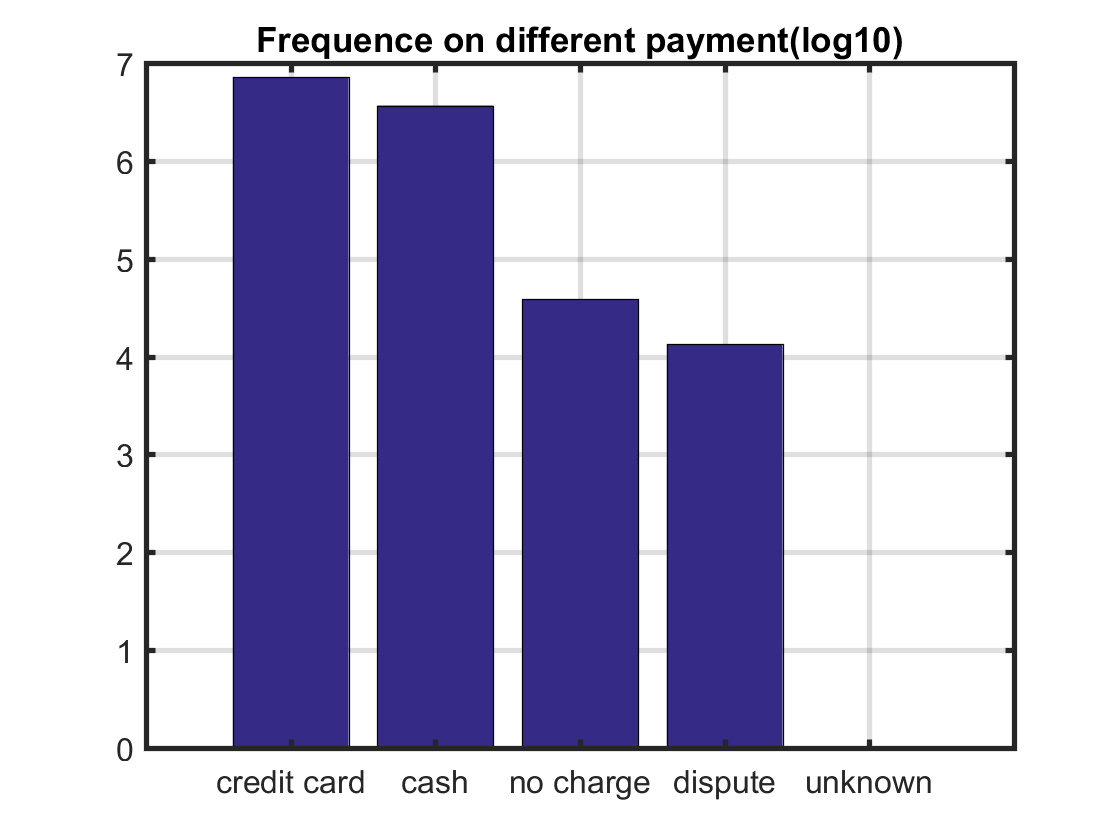
\includegraphics[width=.8\linewidth]{frequency-payment}
  \caption{Frequency of different payment methods}
  \label{sub:payment}
\end{subfigure} & 
\begin{subfigure}{.5\linewidth}
  \centering
  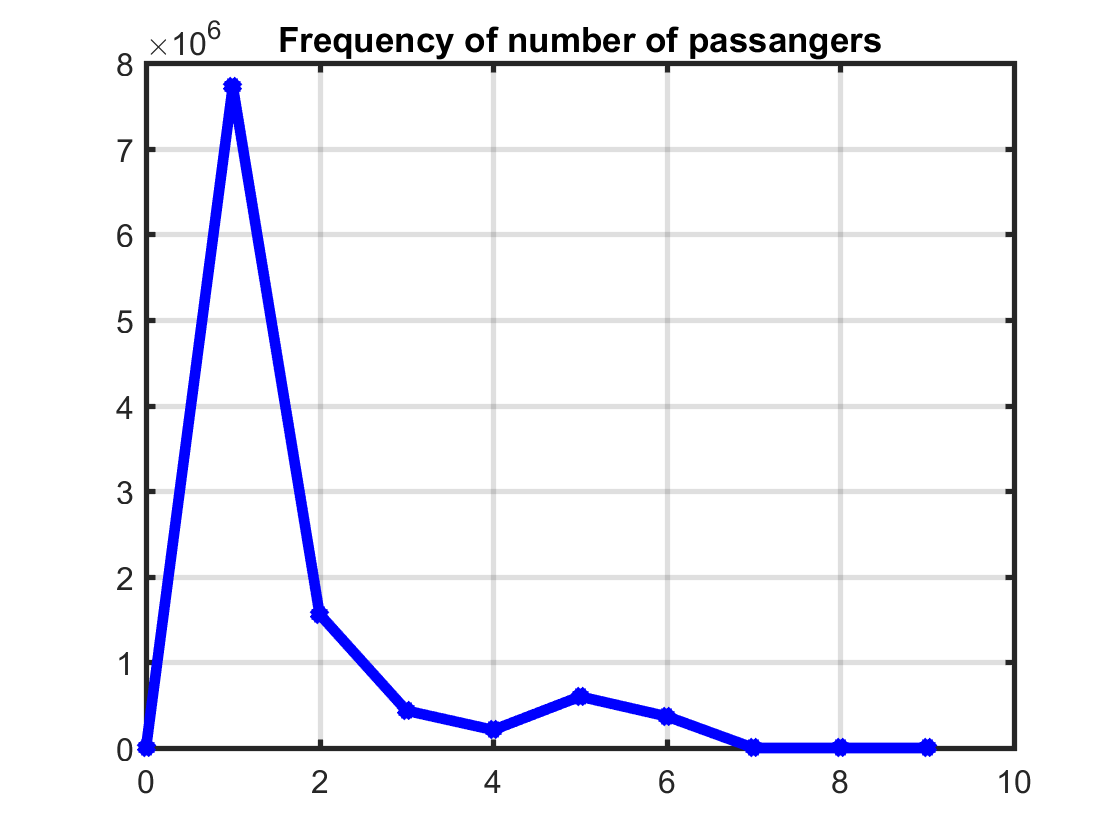
\includegraphics[width=.8\linewidth]{passange_frequency}
  \caption{Frequency of the number of passengers}
  \label{sub:num_pass}
\end{subfigure} \\\\
\begin{subfigure}{.5\linewidth}
  \centering
  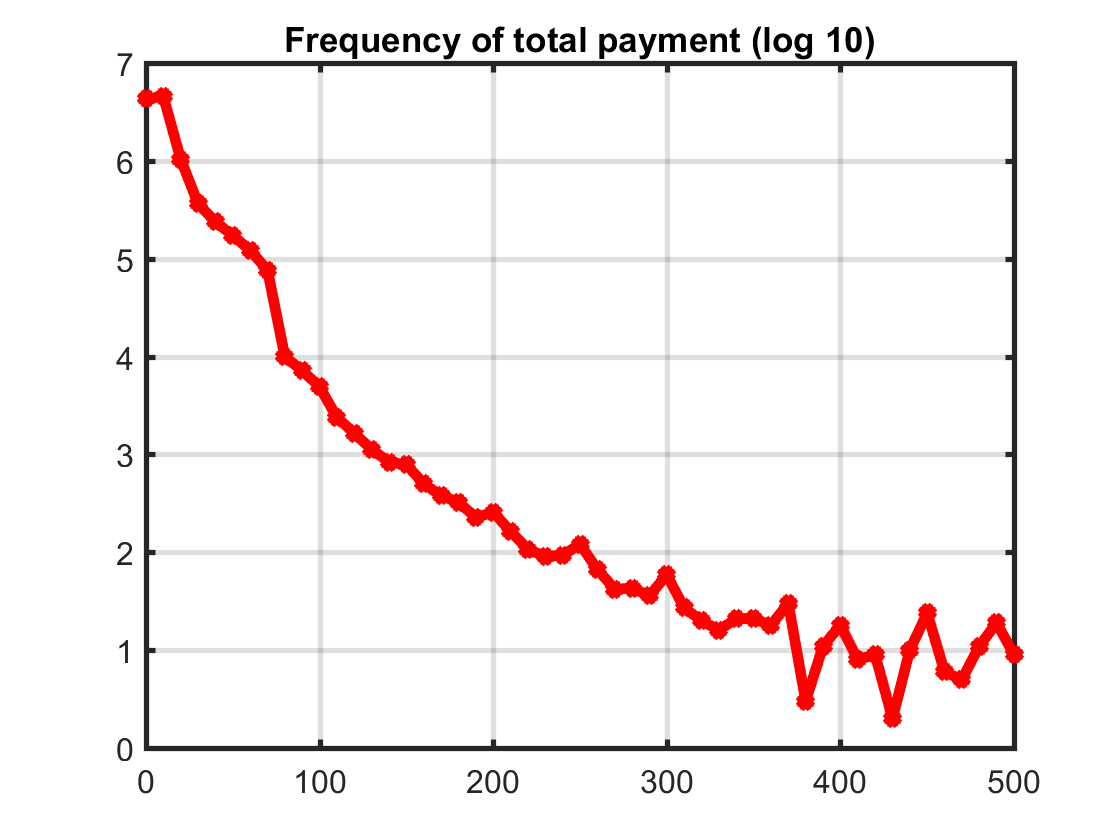
\includegraphics[width=.8\linewidth]{frequency-totalpayment}
  \caption{Frequency of the total payment amount}
  \label{sub:tamount}%
\end{subfigure} &
\begin{subfigure}{.5\linewidth}
  \centering
  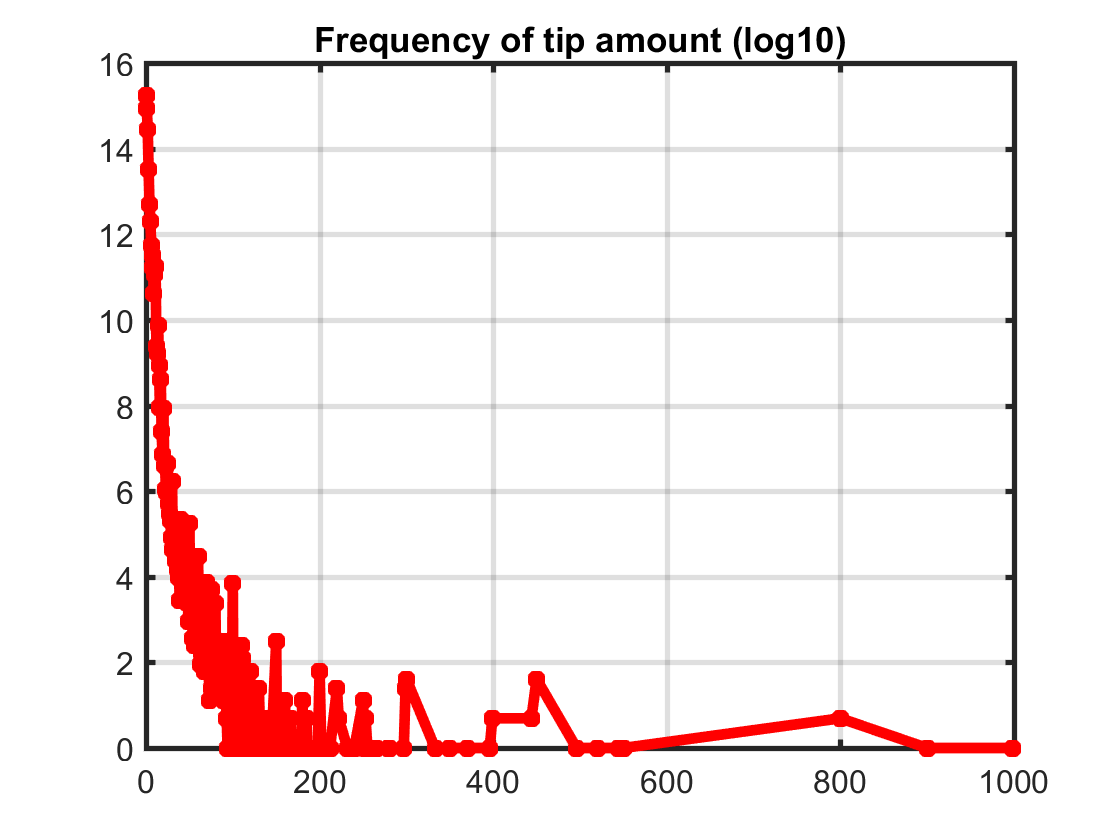
\includegraphics[width=.8\linewidth]{frequency-tipamount}
  \caption{Frequency of the tip amount}
  \label{sub:tip_amount}
\end{subfigure} \\ 

\end{tabular}

\caption{Basic ride statistics}
\label{fig:bstats}
\end{figure}


\subsection{Analysis of the Frequency of Certain Decimal Places in the Price}
The prices of the taxi rides have peculiar distributions that show us a little about human psychology and a lot about the way that the taxi pricing scheme works. From Figure \ref{sub:dec_tip_amount} we can see that the that tips are periodic fluctuations is frequency at numbers that are divisible by 5 and the fare amount (pre-tax / other charges) is divisible by \$$0.50$ over $99.9\%$ of the time  (New Yorkers like round numbers). However, we noticed that the total price paid (Figure \ref{sub:dec_tamount}) is either \$$0.30$ and \$$0.80$ in over $99.9\%$ of taxi rides. We originally thought this must be the MTA Tax that started being levied in 2015, but $99.5\%$ of passengers pay a \$$0.50$ MTA tax. After a good bit of head scratching, we noticed that $99.95\%$ of passengers pay a \$$0.30$ "improvement surcharge" and thus puts the final price at the odd \$$0.30$ or \$$0.80$.


% Figure 2
\begin{figure}[H]
\centering
\begin{subfigure}{.5\linewidth}
  \centering
  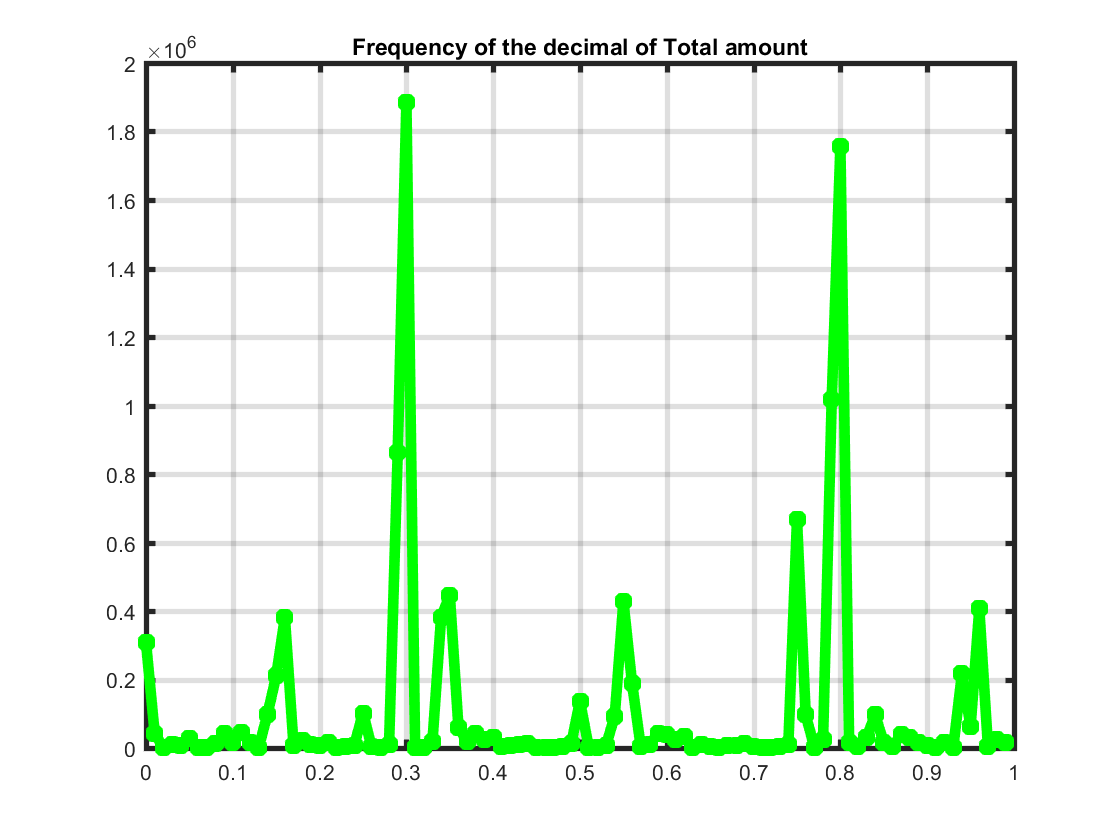
\includegraphics[width=.8\linewidth]{frequency-decimal-totalamount}
  \caption{Frequency of the decimal of total amount paid}
  \label{sub:dec_tamount}
\end{subfigure}%
\begin{subfigure}{.5\linewidth}
  \centering
  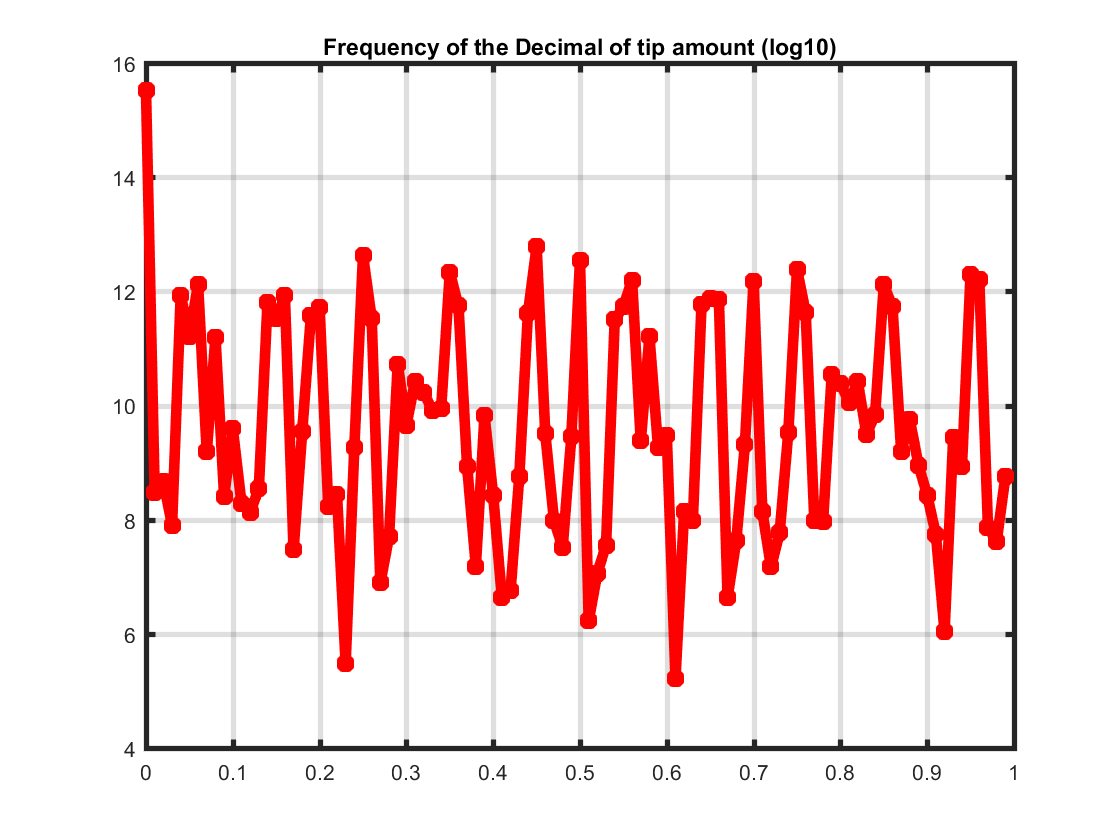
\includegraphics[width=.8\linewidth]{frequency-decimal-tipamount}
  \caption{Frequency of the decimal of tip amount}
  \label{sub:dec_tip_amount}
\end{subfigure}%
\vspace{1cm}
\begin{subfigure}{\linewidth}
  \centering
  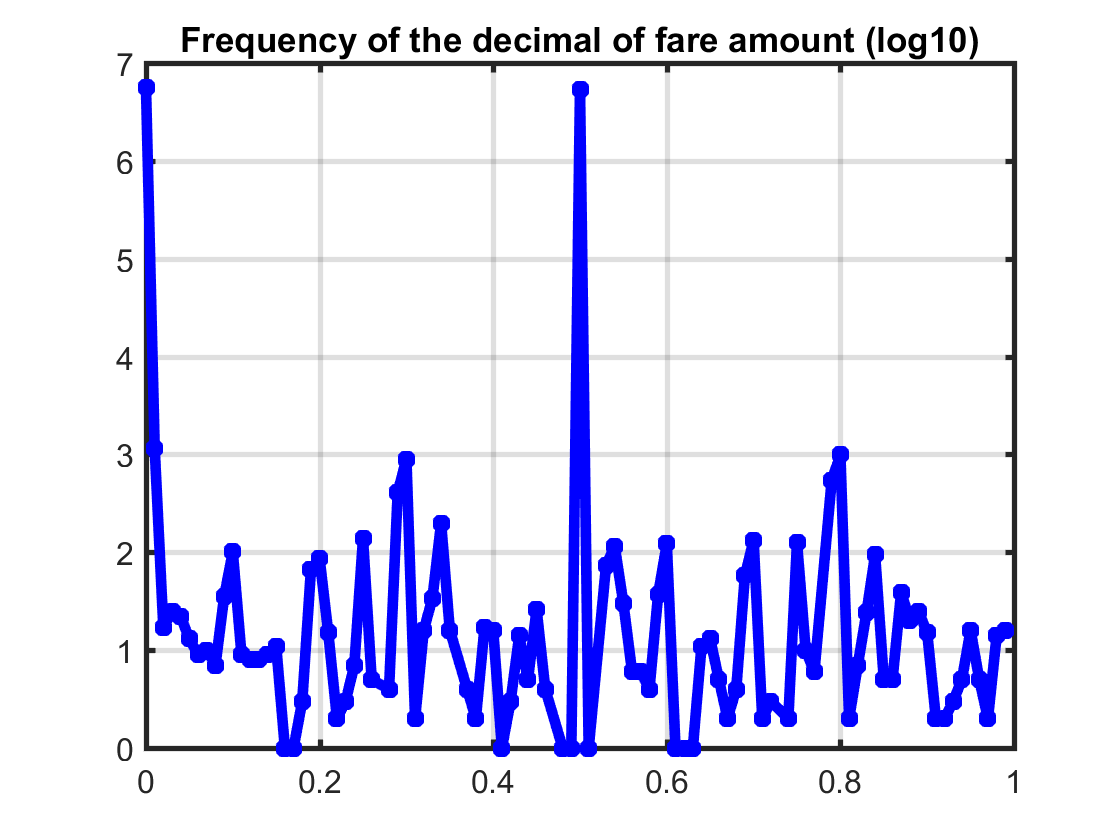
\includegraphics[width=.4\linewidth]{frequency-decimal-fareamount}
  \caption{Frequency of fare amount decimal}
  \label{fig:sub7}
\end{subfigure}%
	
\caption{Frequency of decimal amounts in various parts of the fare}
\label{fig:decimals}
\end{figure}


\subsection{Changes in Ride Characters based on Time of Ride}

Figure \ref{fig:ride_stats} shows the fluctuation of number of rides, average distance of rides and average duration, with respect to the 24 hours in a day, 7 days in a week and 31 days in a month. Our data is from January 2016, so the monthly view shouldn't be taken as an aggregate representation about rides at certain times of the month, but rather a case study of the rides done in January, 2015. In the figure, each subfigure contains two lines with different Y scales. The left column is the numbers of rides or average distance, whereas the right column is number of rides or average duration. The three rows correspond to hours in a day, days in a week and days in a month.

Column-wise, it shows that the average distance shows negative relation with number of rides, while average duration shows positive relation with number of rides. It is intuitive that with more rides, the traffic is heavier thus the average duration increases. It is relatively hard to interpret the negative correlation between number of rides and the average distance of rides. Another interesting finding is the plunge on number of riders around Jan. 23, in the plot of days in month (e,f). This was due to the blizzard that happened on January 22nd, 2016. It took a couple of days for the number of rides to recover after the blizzard. The average distance and average duration also spiked in the days after the blizzard. We hypothesize that some people were displaced / stranded because of the snow and were finally able able to return home, thus increasing average utilization of the taxis. Where utilization is the ratio of the time that all taxis are spent with and without passengers in them. 


% Start of the second Figure
\begin{figure}[H]
\centering
\begin{subfigure}{.5\linewidth}
  \centering
  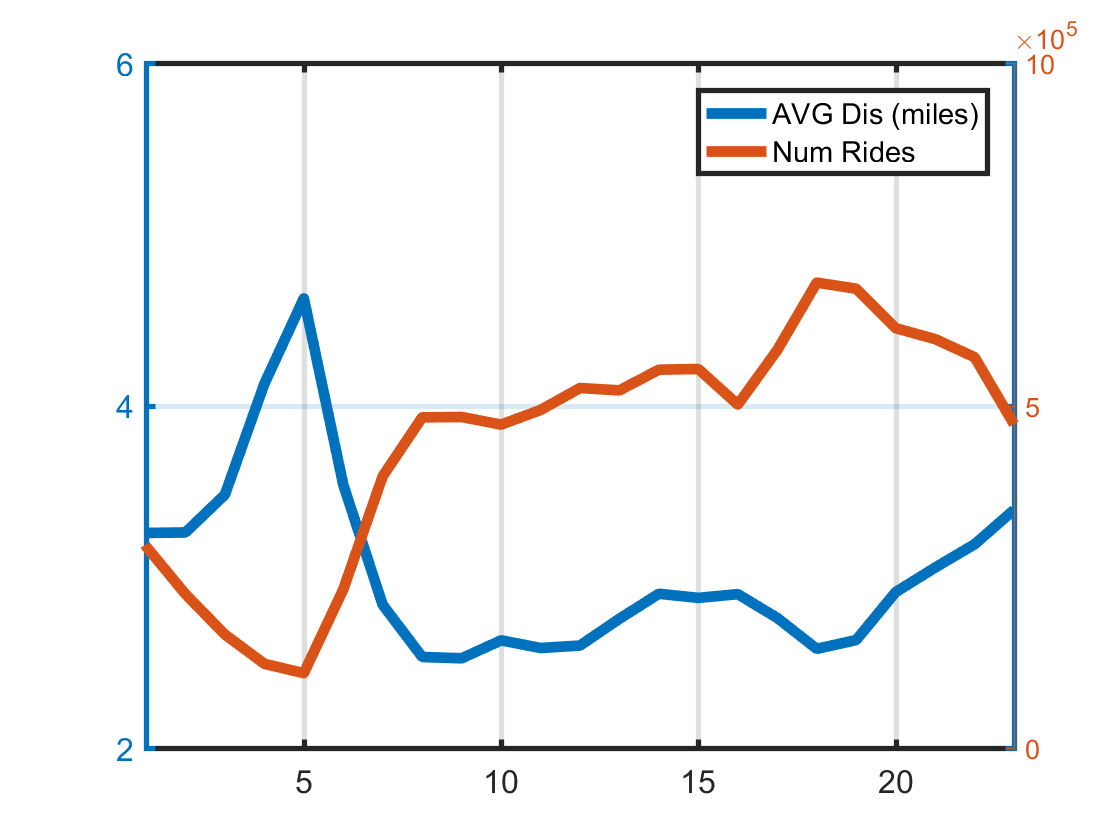
\includegraphics[width=.8\linewidth]{numride_tod}
  \caption{Number of rides \& avg. distance (miles) in 24 hours}
  \label{fig:sub1}
\end{subfigure}%
\begin{subfigure}{.5\linewidth}
  \centering
  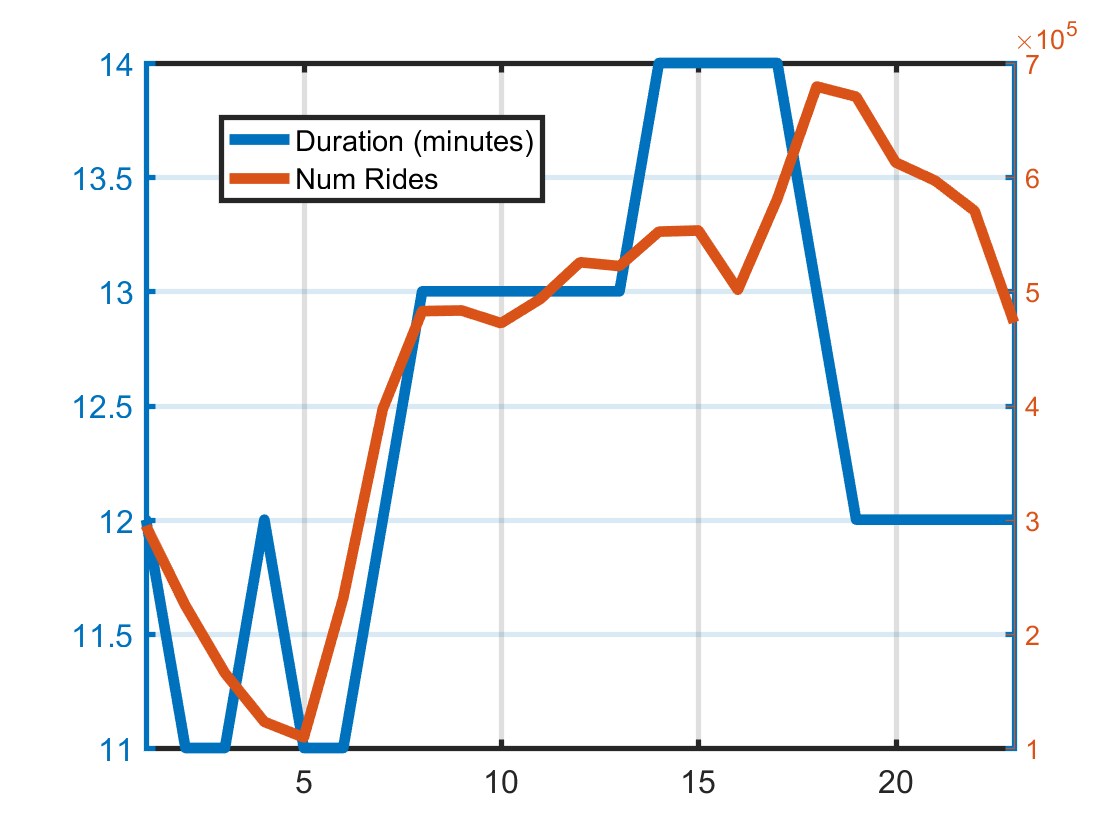
\includegraphics[width=.8\linewidth]{numride_tod_dur}
  \caption{Number of rides \& avg. duration in (min) 24 hours}
  \label{fig:sub2}
\end{subfigure}

\begin{subfigure}{.5\linewidth}
  \centering
  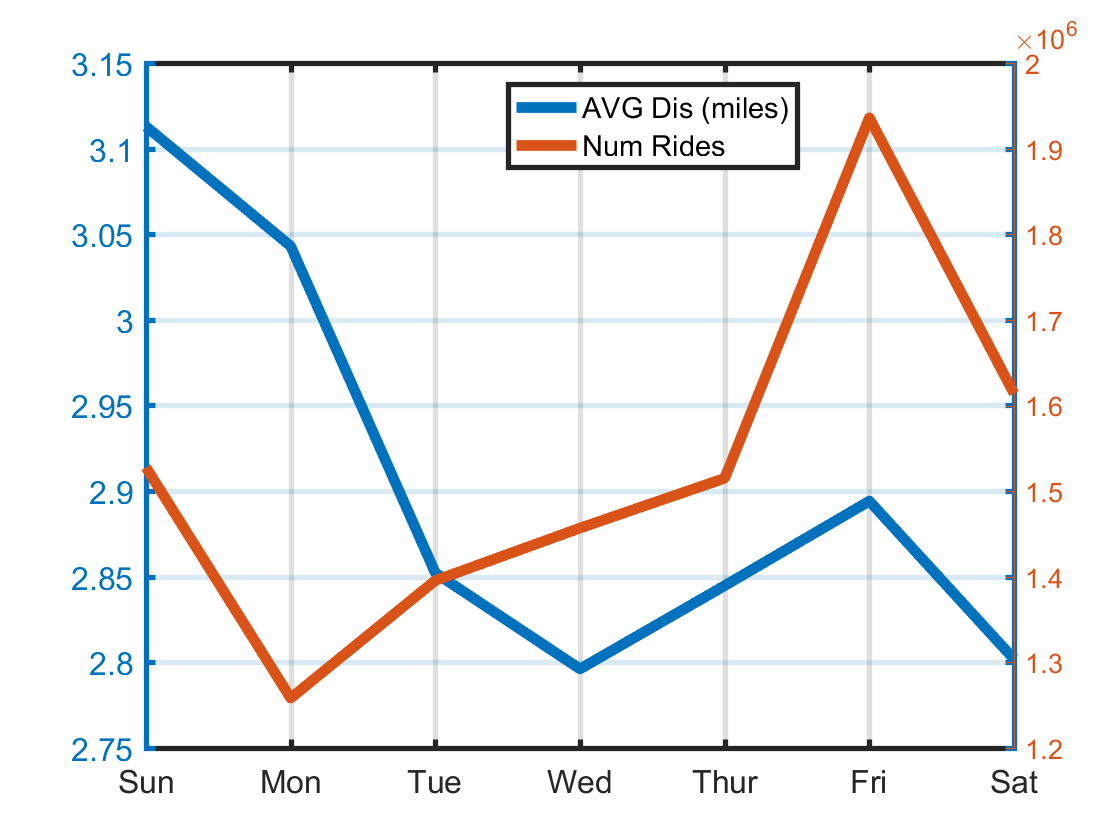
\includegraphics[width=.8\linewidth]{numride_dow}
  \caption{Number of rides \& avg. distance (miles) in 7 days}
  \label{fig:sub3}
\end{subfigure}%
\begin{subfigure}{.5\linewidth}
  \centering
  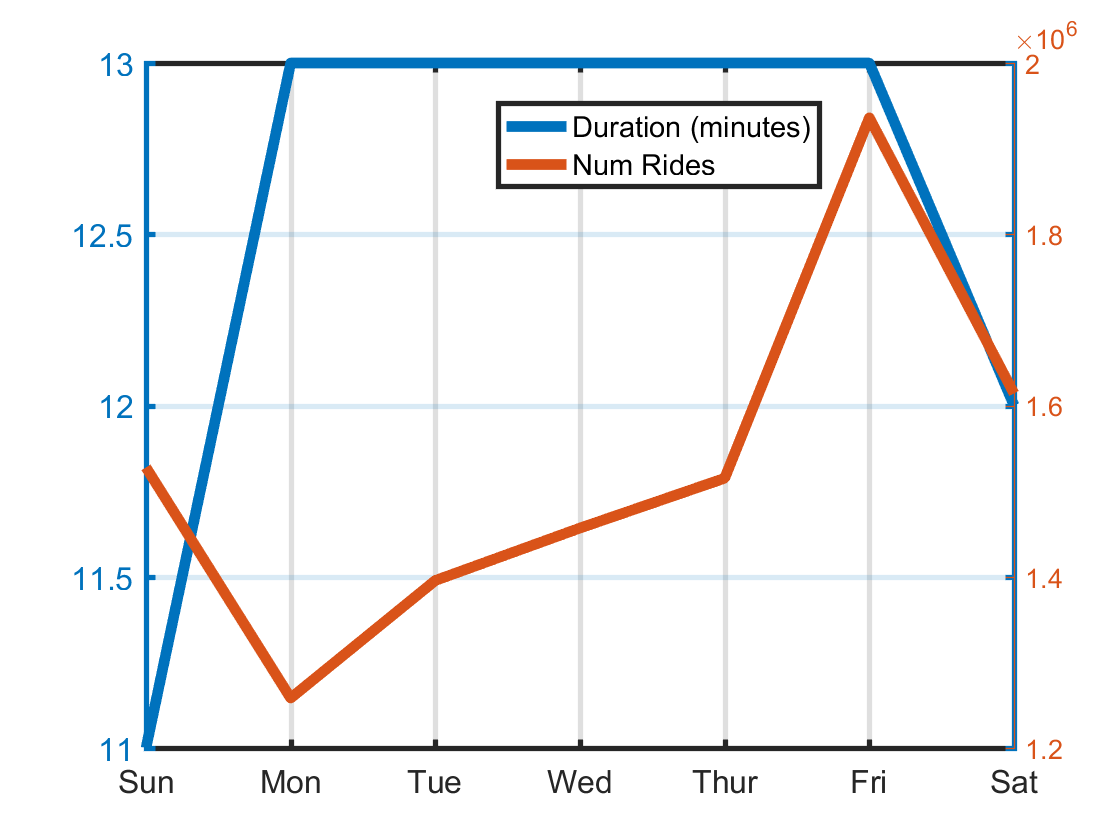
\includegraphics[width=.8\linewidth]{numride_dow_dur}
  \caption{Number of rides \& avg. duration (min) in 7 days}
  \label{fig:sub4}
\end{subfigure}

\begin{subfigure}{.5\linewidth}
  \centering
  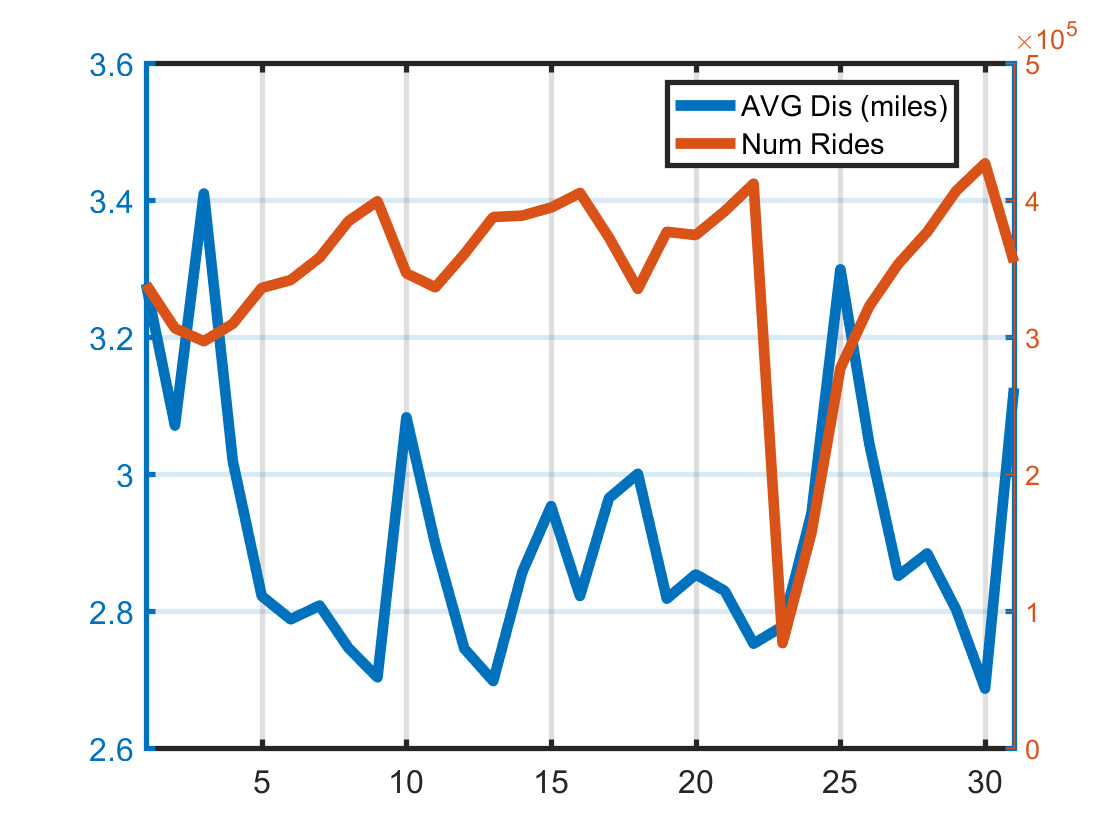
\includegraphics[width=.8\linewidth]{numride_dom}
  \caption{Number of rides \& avg. distance (miles) in 31 days}
  \label{fig:sub5}
\end{subfigure}%
\begin{subfigure}{.5\linewidth}
  \centering
  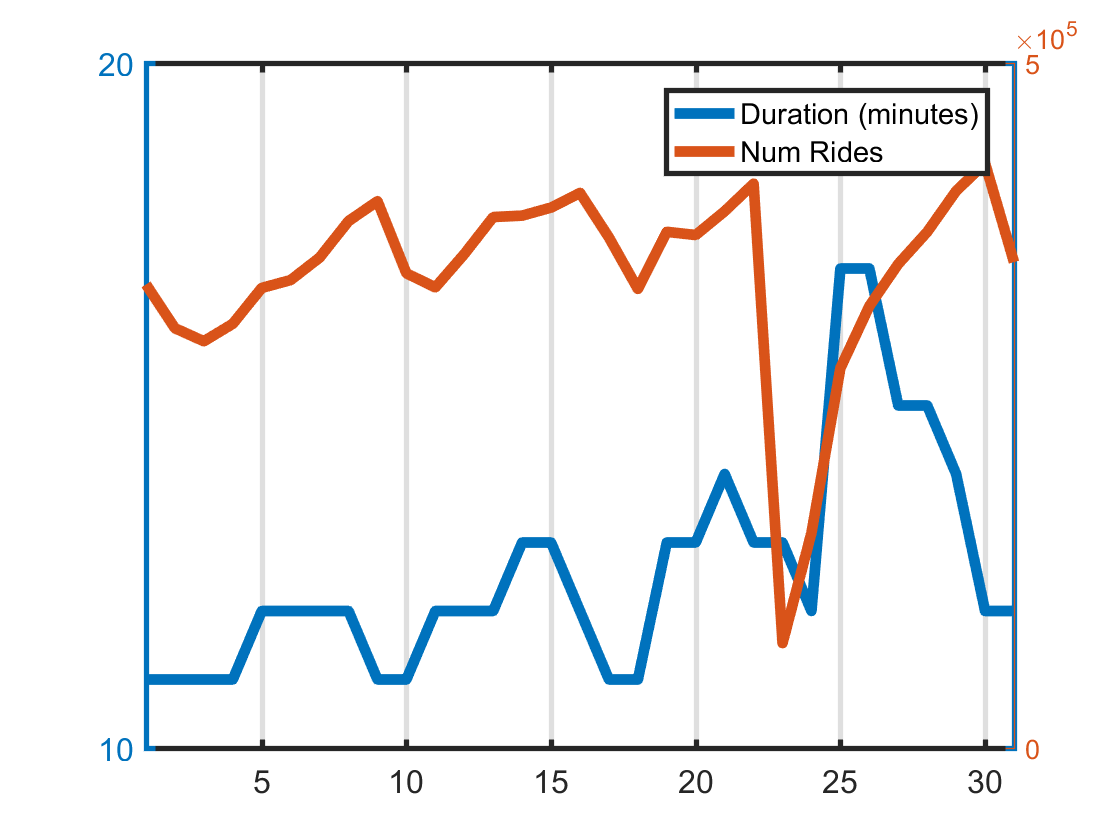
\includegraphics[width=.8\linewidth]{numride_dom_dur}
  \caption{number of ride \& average duration (min) in 31 days}
  \label{fig:sub6}
\end{subfigure}

\caption{Statistics from number of rides, distance and duration}
\label{fig:ride_stats}
\end{figure}

\section{Geographical Visualization of Data}
Given that our dataset is describing how New Yorkers got around, we thought it proper to analyze the frequency of rides as they relate to each other geographically. Figure \ref{fig:heatmap} shows heat maps of the pickup and drop-off locations for the yellow taxi rides from January 2016. Rides around Manhattan are significantly more popular, as most yellow taxis will immediately return after making a drop-off outside the zone. However, as you can see from Figure \ref{sub:do_oh}, the drop-off area for rides is far wider than that of pickups because people can only get a yellow taxi while down-town. 

There are four notable zones of high ride volume: Manhattan and JFK / Laguardia / Newark Airports. Newark airport sees considerably more drop-offs than pickups, while the numbers are fairly similar for Laguardia and JFK. It is unclear from this dataset whether fewer people take a taxi back from Newark than take a taxi to be dropped off or whether there are only fewer yellow taxis that pickup passengers there (for reasons discussed in above paragraph). 

\begin{figure}

\begin{tabular}{cc}

\begin{subfigure}{.5\linewidth}
  \centering
  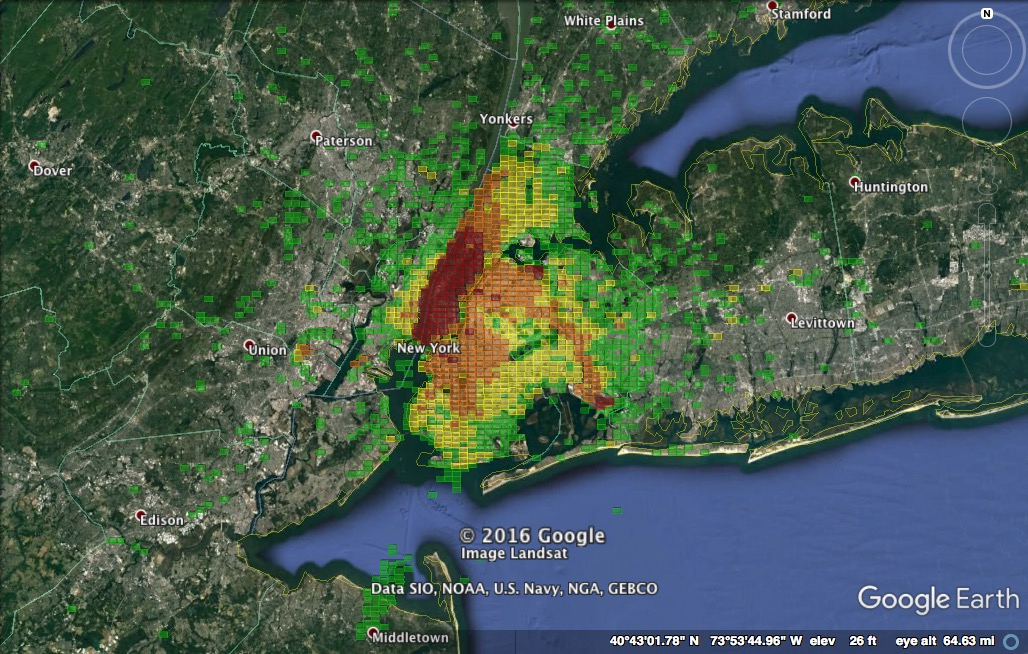
\includegraphics[width=.8\linewidth]{pickup_overhead.jpg}
  \caption{Heatmap of Pickup Locations}
  \label{sub:pu_oh}
\end{subfigure} & 
\begin{subfigure}{.5\linewidth}
  \centering
  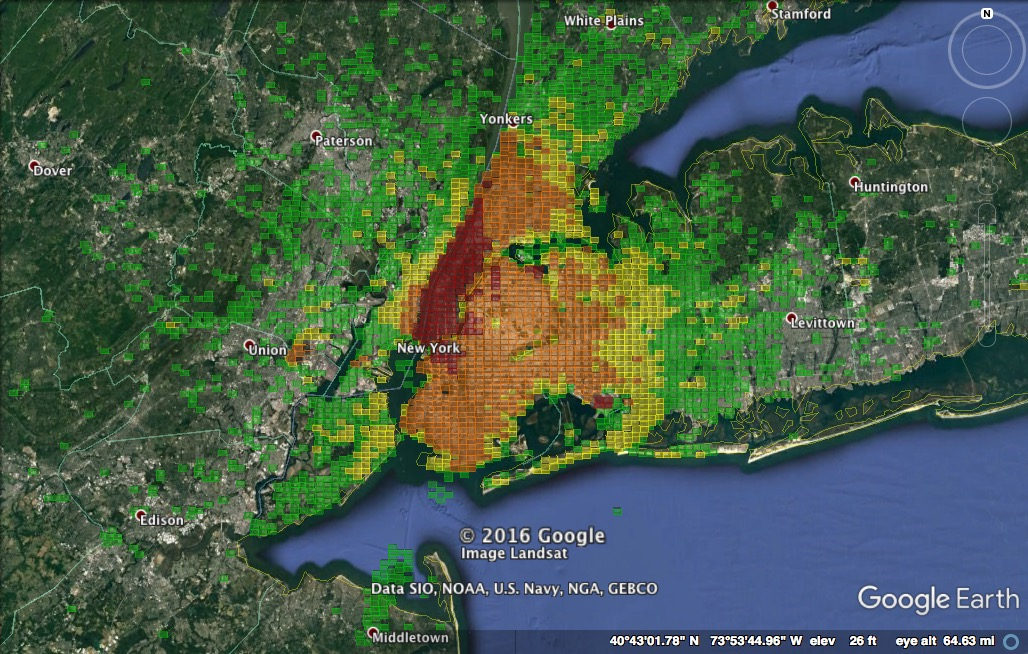
\includegraphics[width=.8\linewidth]{dropoff_overhead.jpg}
  \caption{Heatmap of Drop-off Locations}
  \label{sub:do_oh}
\end{subfigure} \\\\
\begin{subfigure}{.5\linewidth}
  \centering
  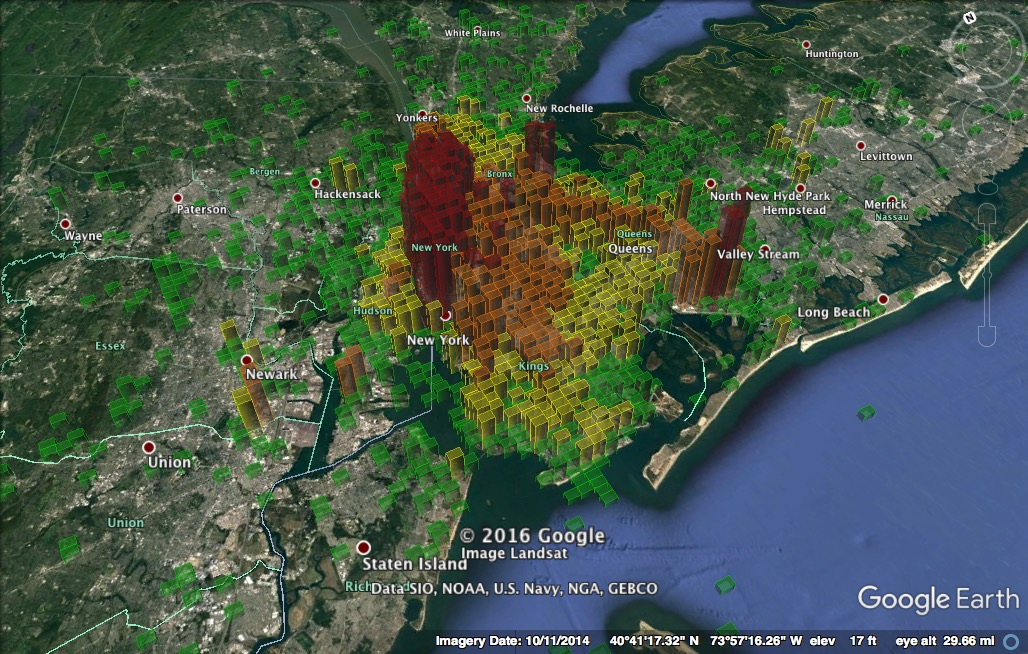
\includegraphics[width=.8\linewidth]{pickup_ne.jpg}
  \caption{Heightmap of Pickup Locations}
  \label{sub:pu_ne}%
\end{subfigure} &
\begin{subfigure}{.5\linewidth}
  \centering
  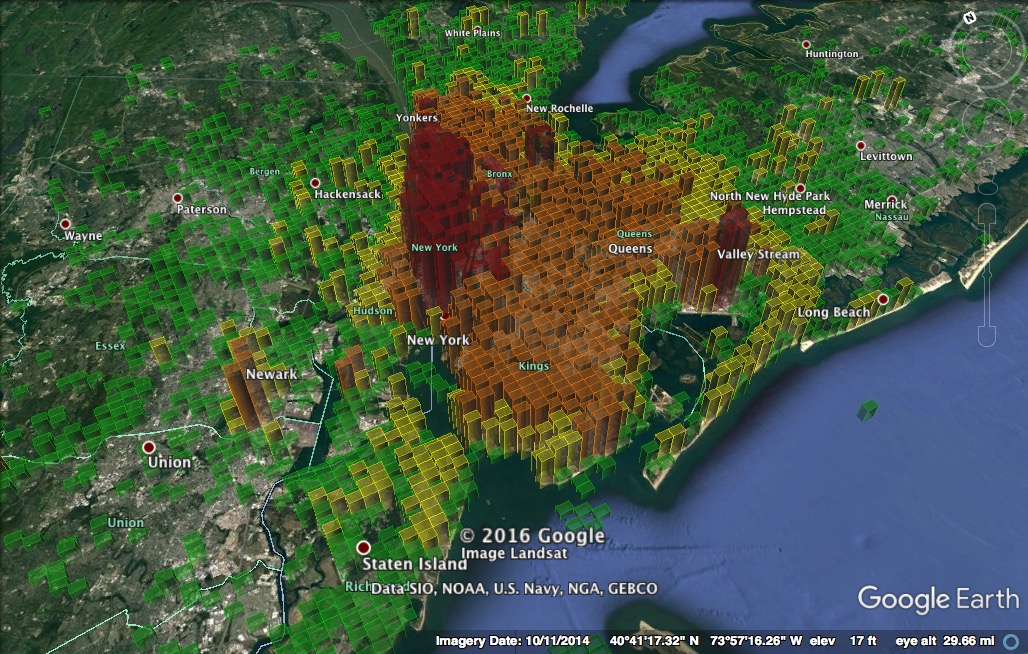
\includegraphics[width=.8\linewidth]{dropoff_ne.jpg}
  \caption{Heightmap of Dropoff Locations}
  \label{sub:do_ne}
\end{subfigure} \\ 

\end{tabular}
\label{fig:heatmap}
\caption{Maps of Activity by type}
\end{figure}

\vfill

\medskip
\bibliographystyle{unsrt}
\bibliography{midterm_report}


\end{document}
\grid
\grid
\grid
